\documentclass[conference]{IEEEtran}
\IEEEoverridecommandlockouts
\usepackage{cite}
\usepackage{amsmath,amssymb,amsfonts}
\usepackage{algorithmic}
\usepackage{graphicx}
\usepackage{textcomp}
\usepackage{xcolor}
\usepackage{threeparttable}
\usepackage{float}
\usepackage{hyperref}

\floatstyle{boxed} 
\restylefloat{figure}

\def\BibTeX{{\rm B\kern-.05em{\sc i\kern-.025em b}\kern-.08em
	T\kern-.1667em\lower.7ex\hbox{E}\kern-.125emX}}
\begin{document}

\title{Sleep State Prediction Using Accelerometry Data: A Systematic and Computational Approach}

\author{
	\IEEEauthorblockN{Juan Carlos Quintero Rubiano}
	\IEEEauthorblockA{Code: 20232020172\\
		\textit{Systems Engineering} \\
		\textit{Francisco Jose de Caldas District University}\\
		Bogota, Colombia \\
		jcquineror@udistrital.edu.co}\\
	%and
	\IEEEauthorblockN{Juan Felipe Wilches Gomez}
	\IEEEauthorblockA{Code: 20231020137\\
		\textit{Systems Engineering} \\
		\textit{Francisco Jose de Caldas District University}\\
		Bogota, Colombia \\
		jfwilchesg@udistrital.edu.co}
	\and
	\IEEEauthorblockN{Juan Nicolas Diaz Salamanca}
	\IEEEauthorblockA{Code: 20232020059\\
		\textit{Systems Engineering} \\
		\textit{Francisco Jose de Caldas District University}\\
		Bogota, Colombia \\
		jndiazs@udistrital.edu.co}
}

\maketitle
\begin{abstract}
	Sleep constitutes a fundamental physiological process comprising multiple distinct states, each fulfilling critical roles in maintaining optimal health and cognitive function. As a highly sensitive biological system, sleep demonstrates exceptional susceptibility to environmental perturbations, whereby subtle variations in ambient conditions, acoustic environments, or external stimuli can substantially influence sleep onset latency, duration, and state transition quality. Conventional sleep state assessment relies predominantly on polysomnography (PSG), a methodology that is both financially prohibitive and clinically intrusive. Contemporary advances in wearable sensor technology have facilitated the utilization of accelerometric devices as non-invasive, cost-effective alternatives for sleep state prediction. This investigation presents a comprehensive systematic analysis and computational framework for predicting sleep states through accelerometric data analysis, emphasizing the extraction of movement patterns and temporal characteristics while accounting for the inherent environmental sensitivity of sleep systems. We examine the theoretical foundations, computational models, and methodological considerations, elucidating both the potential and limitations of accelerometer-based sleep monitoring in capturing environmentally-influenced state transitions.
\end{abstract}

\begin{IEEEkeywords}
	Sleep state classification, accelerometry, computational modeling, wearable sensing technologies, circadian rhythm analysis, temporal feature extraction.
\end{IEEEkeywords}

\section{Introduction}

Sleep represents a fundamental biological process that exerts profound influence on physical health, cognitive performance, and psychological well-being \cite{walker2017we}. Conventional sleep state assessment relies predominantly on polysomnography (PSG), which necessitates simultaneous recording of multiple physiological signals including electroencephalography (EEG), electrooculography (EOG), and electromyography (EMG) \cite{berry2012rules}. However, PSG requires specialized facilities, trained technicians, and sophisticated instrumentation, rendering it financially prohibitive and geographically inaccessible for widespread clinical applications \cite{sadeh2011role}.

The proliferation of wearable sensor technology has facilitated continuous sleep monitoring through actigraphic approaches, which employ accelerometric sensors to quantify movement patterns \cite{ancoli2003role}. The foundational principle establishes that sleep epochs are characterized by markedly reduced motor activity, whereas wake periods demonstrate substantially increased movement amplitude. Contemporary tri-axial accelerometers capture high-resolution acceleration data across three spatial dimensions, providing comprehensive information for robust sleep state inference.

Actigraphy has established itself as a cornerstone technology for non-invasive sleep monitoring, with extensive research validating its effectiveness across diverse populations \cite{smith2018use}. Traditional actigraphic algorithms have dominated the field for decades, with the Cole-Kripke algorithm introducing a weighted scoring system that incorporates current epoch activity and surrounding temporal context \cite{cole1992automatic}. This algorithm demonstrates robust performance in healthy adults, achieving 85-90% accuracy when validated against polysomnography. Concurrently, the Sadeh algorithm represents another foundational approach, originally designed for pediatric populations but adapted for adult applications \cite{sadeh1994activity}. The Sadeh methodology employs different weighting schemes and incorporates variability measures across adjacent epochs \cite{meltzer2012direct}.

Contemporary developments have introduced sophisticated approaches transcending traditional activity counting paradigms. The OPAL algorithm represents significant advancement by incorporating postural information alongside activity metrics \cite{hickey2021smart}. Machine learning methodologies have been progressively applied to actigraphic data, demonstrating substantial accuracy improvements through feature engineering and ensemble approaches \cite{beattie2017estimation}. Recent advances in artificial intelligence have demonstrated the potential of Large Language Models (LLMs) for time series analysis applications, exhibiting remarkable capabilities in pattern recognition and temporal sequence modeling that translate to physiological signal analysis \cite{jin2023time}. The attention mechanisms in transformer architectures enable capture of long-range temporal dependencies, particularly relevant for circadian rhythm analysis \cite{zhou2023onellm}.

Comprehensive evaluations reveal substantial variations in classification performance across different populations and sleep conditions \cite{martin2011wrist}. The Cole-Kripke algorithm typically demonstrates superior performance in healthy adults with regular sleep patterns, while the Sadeh algorithm shows better sensitivity for detecting sleep fragmentation \cite{cellini2013direct}. Contemporary research emphasizes the importance of personalized algorithm calibration, recognizing that individual differences significantly impact classification accuracy \cite{koesmahargyo2019accuracy}.

This investigation presents a systematic computational approach for predicting sleep states utilizing accelerometric data from wearable devices. Our framework encompasses comprehensive data preprocessing, sophisticated feature extraction, and application of both traditional and contemporary computational models for sleep-wake classification, providing a comprehensive framework for accelerometer-based sleep state prediction.

\section{Method and Materials}

The development of our sleep state prediction system followed a systematic three-phase approach, beginning with comprehensive system analysis, followed by architectural design, and culminating in behavioral simulation studies. This methodology ensured a thorough understanding of the problem domain while establishing robust technical foundations for the proposed solution.

During the initial workshop phase, we conducted an extensive systems analysis to identify the fundamental components and interactions within sleep monitoring ecosystems. This analysis revealed the complex interplay between physiological signals, environmental factors, and technological constraints that characterize sleep state detection systems. We identified several sources of chaos and uncertainty within traditional sleep monitoring approaches, including signal artifacts from movement, environmental perturbations affecting sleep quality, and the inherent variability in individual sleep patterns. The systems perspective highlighted the need for adaptive algorithms capable of handling these dynamic interactions while maintaining classification accuracy across diverse populations and conditions.

As illustrated in Figure \ref{fig:workshop1_analysis}, the initial systems analysis revealed the fundamental data flow architecture that would guide our subsequent design decisions. The diagram shows the identification of key input sources including EMMO acceleration data, angle-based measurements from body position, step counting, and timestamp event recording. The central processing components identified include a data preprocessor for signal conditioning, an event detection module for identifying sleep-wake transitions, and dedicated wake-up and sleep state classifiers. The analysis also revealed the critical importance of validation mechanisms and pattern recognition elements to ensure system reliability and accuracy.

\begin{figure}[htbp]
	\centering
	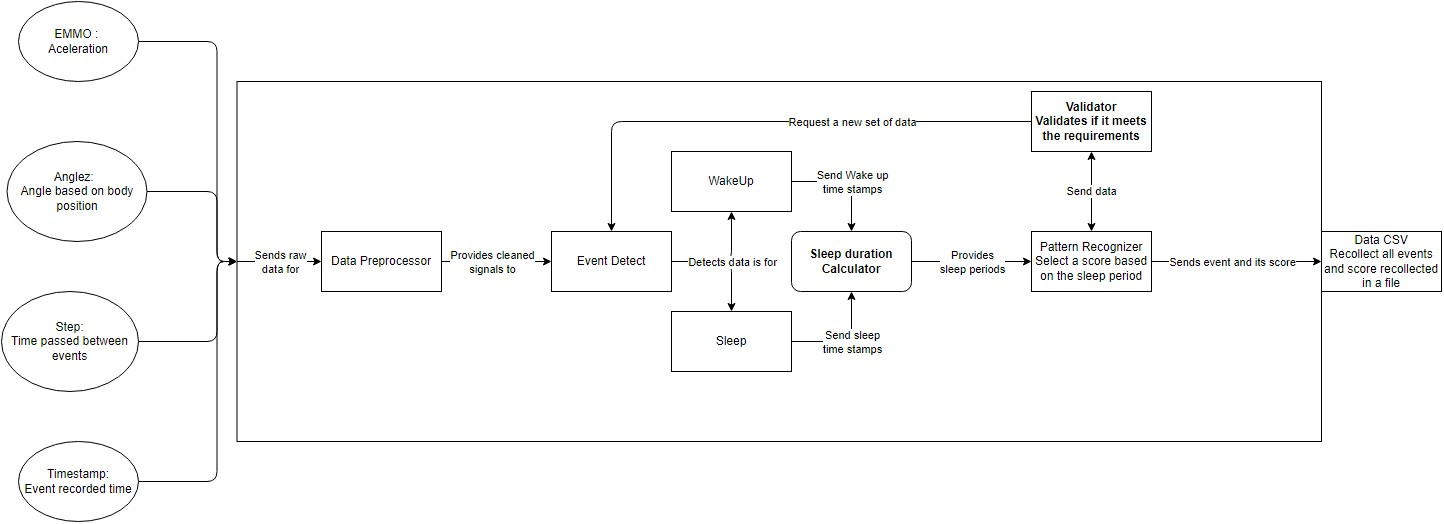
\includegraphics[width=\columnwidth]{system_analysis_workshop1.png}
	\caption{Initial systems analysis from Workshop 1 showing the identification of key components, data flows, and processing stages in the sleep monitoring ecosystem, including validation mechanisms and pattern recognition elements.}
	\label{fig:workshop1_analysis}
\end{figure}

The second workshop phase focused on architectural selection and system design, where we evaluated multiple computational architectures before selecting a modular approach as the most suitable solution for our problem domain. As demonstrated in Figure \ref{fig:architecture}, the modular architecture was chosen due to its inherent flexibility, scalability, and maintainability advantages over monolithic approaches, directly informed by the information flow analysis conducted in Workshop 1. This architecture enables independent development and optimization of individual components while facilitating seamless integration and data flow between modules.

Our proposed system architecture comprises five interconnected modules that systematically address the sleep state prediction challenge through a data transformation pipeline. The Data Acquisition module manages the collection and initial processing of accelerometric data from wearable devices, ensuring timestamp synchronization and basic quality assessment. The Data Processing module performs signal conditioning, including calibration, normalization, filtering, and gap detection, to transform raw measurements into analysis-ready datasets. The Feature Extraction module implements algorithms to obtain relevant temporal and frequency descriptors from the preprocessed signals. The core of this analysis is the calculation of the activity count:

\begin{equation}
	\scriptsize
	AC_{epoch} = \sum_{j=1}^{N} ENMO_j \times 1000
\end{equation}
where $AC_{epoch}$ is the activity count for each epoch, $ENMO_j$ is the ENMO value at step $j$ within the epoch, $N$ is the number of steps per epoch, and the factor 1000 is a typical scaling to facilitate interpretation. This metric summarizes physical activity during the period and serves as the basis for sleep/wake classification.

The Classification module is the core intelligence of the system, implementing both traditional methods such as Cole-Kripke and Sadeh, and contemporary machine learning techniques. Finally, the Sleep State Prediction module integrates classification results with temporal sequence analysis to generate robust predictions, incorporating validation mechanisms to ensure quality and reliability.


This modular architecture is illustrated in Figure~\ref{fig:architecture}, which shows the five modules and their information flow. This organization enables independent development and validation of each component, facilitates the integration of new algorithms, and supports both real-time and offline analysis, adapting to clinical and research environments.



\begin{figure}[htbp]
	\centering
	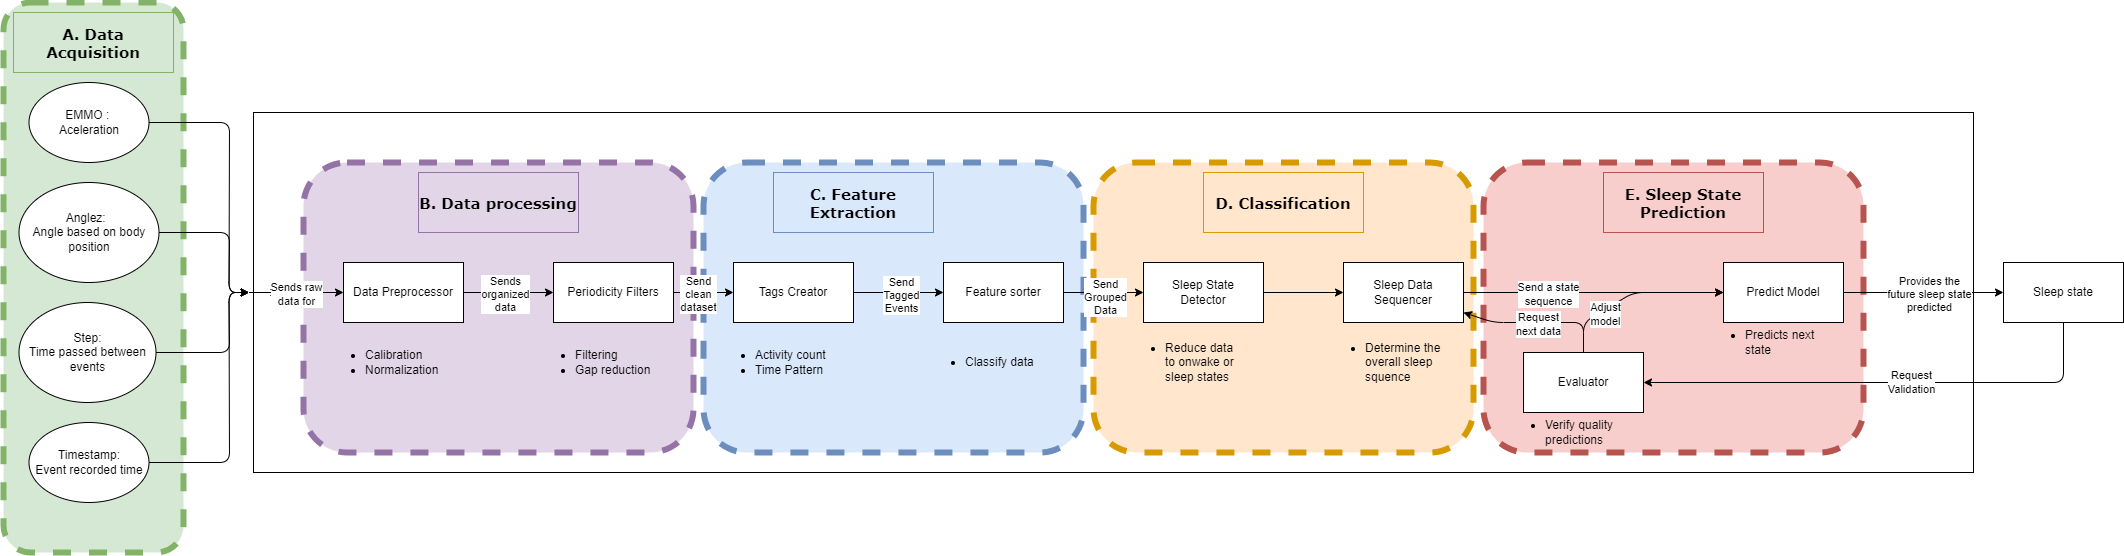
\includegraphics[width=\columnwidth]{system_architecture.png}
	\caption{Modular architecture for sleep state prediction system showing the five interconnected modules: Data Acquisition, Data Processing, Feature Extraction, Classification, and Sleep State Prediction.}
	\label{fig:architecture}
\end{figure}

The algorithms implemented include:

\textbf{Cole-Kripke:}
\begin{equation}
	\scriptsize
	S_i = \frac{0.04\,AC_{i-2} + 0.20\,AC_{i-1} + 2.00\,AC_i + 0.20\,AC_{i+1} + 0.04\,AC_{i+2}}{6.48}
\end{equation}
Based on the score $S_i$, it is classified as sleep ($1$) if $S_i < 1.0$, or wake ($0$) otherwise.


\textbf{Sadeh:}
\begin{equation}
	\scriptsize
	PS_i = 7.601 - 0.065\,AC_i - 1.08\,NAT_i - 0.056\,SD_i - 0.703\,\log(AC_i + 1)
\end{equation}
It is classified as sleep ($1$) if $PS_i \geq 0$, or wake ($0$) otherwise.

\textbf{OPAL:}
\begin{equation}
	\scriptsize
	Z_i = -1.0 - 2.5\,\log(AC_i + 1) + 1.5\,(1 - \frac{SD_i - P_5}{P_{95} - P_5})
\end{equation}
It is classified as sleep ($1$) if $Z_i > 0$, or wake ($0$) otherwise.


\begin{figure}[htbp]
	\centering
	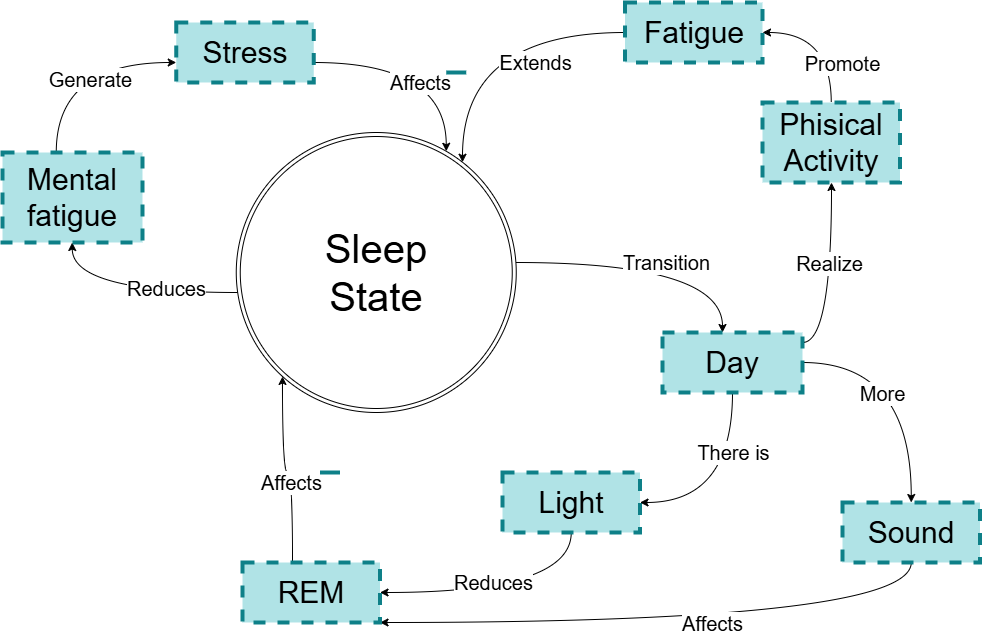
\includegraphics[width=0.85\columnwidth]{simulation.png}
	\caption{Flywheel diagram outlining the interaction between environmental factors and the sleep state. The simulation models how stress, fatigue, physical activity, light, sound, and other contextual variables dynamically influence the probability of being asleep. This probability is then used to generate synthetic ENMO and Anglez data, providing a realistic approximation of actigraphic signals for algorithm evaluation.}
	\label{fig:flywheel_simulation}
\end{figure}

The simulation phase is based on this flywheel model (Figure~\ref{fig:flywheel_simulation}), which sketches the dynamic interplay between environmental and physiological factors and the sleep state. Each factor modulates the probability of being asleep at a given epoch, capturing the multifactorial nature of real-world sleep. This probability is then mapped to synthetic actigraphic signals: ENMO (activity) and Anglez (posture), using empirically derived distributions and noise models. This approach enables the generation of realistic, labeled time series for robust algorithm development and benchmarking, bridging the gap between theoretical modeling and practical data-driven evaluation.

The implementation was carried out in a Python notebook environment, structured into dedicated modules for data loading, preprocessing, feature extraction, and evaluation. The workflow leverages pandas and polars for efficient data manipulation, NumPy for numerical operations, and matplotlib with seaborn for comprehensive visualization. Custom functions were developed to implement the actigraphic algorithms, ensuring transparency and reproducibility. This modular structure mirrors the conceptual architecture, facilitating clarity, reproducibility, and future extensibility.

To realistically assess the robustness of the proposed system, the simulation phase explicitly modeled the influence of key environmental factors—including light intensity, ambient sound, psychological stress, and physical activity—on sleep-wake movement patterns. Environmental disturbances were represented as discrete stochastic events, dynamically modulating the probability of movement during sleep-wake transitions. This event-based framework reflects the complex interplay between environmental stimuli and physiological responses, providing a robust platform for evaluating algorithmic performance under diverse, real-world scenarios. The methodological decision to incorporate these factors is grounded in the recognition that sleep is highly sensitive to external perturbations, and that accurate prediction systems must account for the multifaceted nature of real-life sleep environments.

In the final implementation phase, Amazon's Chronos forecasting model \cite{ansari2024chronos} was integrated to enhance prediction capabilities beyond traditional actigraphic methods. Chronos, a pre-trained transformer-based foundation model for time series forecasting, enables the system to capture complex temporal patterns and long-range dependencies in sleep-wake cycles. The model processes preprocessed accelerometric features and generates probabilistic forecasts of sleep state transitions, providing uncertainty quantification alongside point predictions. This integration combines the interpretability of traditional actigraphic methods with the advanced pattern recognition capabilities of modern foundation models, significantly improving the system's predictive accuracy and adaptability.

For evaluation, the model is used to predict the sleep state for 60 consecutive epochs, corresponding to a 5-minute window (as the recommended maximum for the model is 64 steps). These predictions are then directly compared to the ground truth binary series obtained from the traditional algorithms, allowing for a precise assessment of forecasting accuracy.

\section{Results}



\bibliographystyle{IEEEtran}
\bibliography{references}

\end{document}